% ---------------------------------------------------
%
% Trabajo de Fin de Grado. 
% Author: Alejandro Hernández Padrón. 
% Capítulo: Tecnologías utilizadas en el Trabajo de Fin de Grado. 
% Fichero: Cap2_Technology.tex
% 
% ----------------------------------------------------
%

% \lstset{
%   showstringspaces=false,
%   commentstyle=\color{red},
%   keywordstyle=\color{blue},
%   numbers=none,
%   language=bash,
%   caption={bash version},
%   morekeywords={sudo, apt, curl, node}
% }

\cleardoublepage
\chapter{Herramientas y Tecnologías} \label{chap:Tecnologias} 

Este capítulo tiene como objetivo presentar las distintas herramientas software y tecnologías empleadas por el alumno en el desarrollo de la aplicación Android 
objeto de este TFG. En adelante usaremos el nombre \ULLAR{} para referirnos a la misma.

\section{Herramientas de Desarrollo}

\subsection{Android Studio}

Android Studio \cite{URL::AndroidStudio} es el IDE  \cite{URL::IDE} (Entorno de Desarrollo Integrado) oficial para el desarrollo de aplicaciones en Android, basado en IntelliJ IDEA \cite{URL::IntelliJIDEA}. Android Studio ofrece una serie de funcionalidades que han facilitado al desarrollador numerosas tareas, entre las cuales se pueden destacar:

\begin{itemize}
\item Un sistema de compilación basado en Gradle \cite{URL::Gradle} que ha simplificado tanto la inserción de dependencias de las distintas librerías que se han tenido que utilizar, como la compilación de la aplicación.
\item Un emulador rápido y fácil de utilizar que ha ayudado a visualizar las distintas pantallas durante el desarrollo, el cual ha sido utilidad en las primeras ventanas de la aplicación.
\item La facilidad y velocidad para aplicar cambios a aplicaciones ya funcionando. 
\item Un sistema de visualización de las diferentes pantallas muy completo, con soporte visual para añadir componentes y cambiar atributos fácilmente.
\item Un sistema de depuración, con una interfaz sencilla e intuitiva.
\end{itemize} 

\begin{figure}[h]
    \centering
    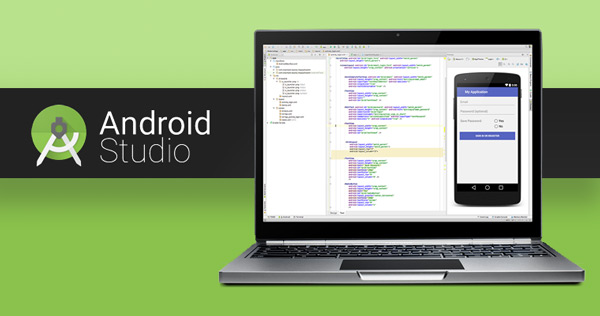
\includegraphics[width=0.6\linewidth]{androidstudio}
    \caption{Android Studio, un IDE flexible e intuitivo.}
    \label{fig:androidstudio}
\end{figure}

\subsection{LaTex}

LaTeX \cite{URL::LaTeX} es un sistema de composición de textos, orientado a la creación de documentos que presenten una alta calidad tipográfica. Por sus características y posibilidades, es usado especialmente en la generación de artículos y publicaciones científicas que incluyen, entre otros elementos, expresiones matemáticas, gráficos o figuras.

LaTeX está formado por un gran conjunto de macros de TeX, escrito por Leslie Lamport en 1984, con la intención de facilitar el uso del lenguaje de composición tipográfica, creado por Donald Knuth. LaTeX es software libre bajo licencia LPPL.

Se ha decidido usar esta herramienta debido a la calidad profesional de los documentos que es posible generar con ella. 
Otra de las ventajas de LaTeX es que permite separar el formato y el contenido del documento, lo cual permite concentrar el esfuerzo en la creación del contenido sin tener que ocuparse del diseño. 

\vskip 0.5in

\subsection{Github}

GitHub \cite{URL::Github} es una plataforma de desarrollo colaborativo para alojar proyectos que utiliza el sistema de control de versiones Git. 
GitHub fue escrito en Ruby on Rails. 
El código se almacena de forma pública, aunque también se puede hacer de forma privada, creando una cuenta de pago.

Se ha decidido crear un repositorio \cite{URL::repositorioAplicacion} en esta plataforma para poder llevar un control y una trazabilidad del proyecto \ULLAR{}. 
El tutor y el alumno han trabajado en este repositorio de manera conjunta. 
En el caso del tutor, principalmente para revisar el seguimiento semanal y llevar un control de las tareas. 
En el caso del alumno, para tener un repositorio donde subir los distintos elementos que se han ido generando a lo largo del trabajo. 
% Aparte de este repositorio, también se ha abierto un segundo repositorio \cite{URL::repositorioAplicacion} asociado a la oficina del software libre (OSL) para subir el código una vez terminado como parte del programa de apoyo a trabajos finales libres (PATFL) \cite{URL::PATFL} de la ULL.
En el repositorio del proyecto \cite{URL::repositorioAplicacion} están disponibles públicamente todos los ficheros necesarios para la elaboración con LaTeX de esta memoria, 
los ficheros correspondientes a la
presentación para la defensa de este TFG así como el proyecto de Android Studio que contiene el código fuente de \ULLAR{}. 

Mediante el uso de este repositorio, el alumno ha conseguido ampliar sus conocimientos en Git y familiarizarse con la interfaz de GitHub.

Para instalar GitHub en Linux se utiliza el siguiente comando:
\begin{lstlisting}
    sudo apt install git-all
\end{lstlisting}

\subsection{Guía de uso de estas tecnologías en relación con el proyecto \ULLAR{}}
En este apartado se explica con cierto nivel de detalle los pasos a seguir para:
\begin{itemize}
\item Descargar desde su repositorio todo el código fuente, tanto de esta memoria como de la aplicación \ULLAR{}.
\item Compilar en Android Studio el proyecto \ULLAR{} para generar una aplicación para dispositivos móviles.
\item Compilar con Latex esta memoria para generar el corresponidente fichero en formato PDF.
\end{itemize}

\subsubsection{Descargar repositorio de la aplicación}

Para descargar el repositorio de \ULLAR{} se necesitará tener instalado GitHub. Con GitHub instalado, se ejecuta el siguiente comando en consola para descargar el repositorio:

\begin{lstlisting}
    git clone https://github.com/alehdezp/TFG-ULL-AR 
\end{lstlisting}

En caso de que no se disponga de GitHub se puede descargar directamente desde el repositorio \cite{URL::repositorioAplicacion}, seleccionando el bóton ``Clone or download'' y luego se selecciona ``Download as ZIP''. Tras esto se descargará un archivo comprimido con todo el repositorio de \ULLAR{}.


\subsubsection{Compilar el proyecto en Android Studio}

Para compilar el proyecto es necesario tener instalado el IDE de Android Studio en el ordenador que se desee compilar el proyecto.

Una vez iniciado Android Studio, se indica que se quiere abrir un proyecto y se busca en la carpeta en la que se encuentra el repositorio de \ULLAR{} y se abre el proyecto que se encuentra en la ruta \textit{``app/ULL\_Navigation''}. 

La primera vez que se abre el proyecto, en el caso de que no se haya hecho automáticamente, se ha de seleccionar en la barra superior la opción de ``Build'' y luego ``Make Project''. 
Esto creára y configurará el proyecto para que se pueda empezar a trabajar con él.

Para poder instalar la aplicación que genera el proyecto en un dispositivo Android hay dos opciones. 
La primera es generar un archivo ``.apk''. Para generar este archivo se ha de seleccionar en la barra superior la opción ``Build'', luego ``Build Bundle(s) / APK(s)'' y por último ``Build APK''. 
Esto generará un fichero \texttt{app-debug.apk} en la ruta \textit{``ULL\_Navigation/app/build/outputs/apk/debug''}, este fichero hay que colocarlo dentro del dispositivo Android en el que se quiera instalar la aplicación y se ejecuta.

La seguna opción es ejecutar e instalar directamente la aplicación desde Android Studio. 
Para ello hay que tener activado en el dispositivo Android la opción de depuración por USB. 
Esta opción solo estará disponible cuando se tenga activado el modo desarrollador en el dispositivo Android. 
En función de la marca y modelo del dispositivo la forma en la que se activa este modo varía. 
Con la opción activada solo hay que conectar el dispositivo al ordenador y seleccionar en el móvil el modo de ``Transeferencia de archivos'', a continuación en Android Studio se selecciona la opción ``Run'' y luego ``Run 'app'''. 
Con estos pasos ya instalará la aplicación en el dispositivo y se solicitarán permisos en el dispositivo móvil para confiar en el desarrollador e instalar la aplicación \ULLAR{}. 


\subsubsection{Compilar la memoria del proyecto}
Para compilar el proyecto en LaTeX en un máquina con Linux es necesario instalar ``TeX Live'' y ``make''. Con el siguiente comando se instalarán ambos:
\begin{lstlisting}
    sudo apt install texlive-full make 
\end{lstlisting}

Dentro de la carpeta \textit{``Memoria/''} del repositorio, se abrirá una consola y se ejecutará el siguiente comando el cual genera el archivo con la presente memoria \texttt{memoria-TFG-Alejandro.pdf}.
\begin{lstlisting}
    make
\end{lstlisting}


\section{Tecnologías utilizadas}

A continuación, se revisan las distintas tecnologías utilizadas en el desarrollo de la aplicación.

\subsection{El Sistema Operativo Android}

Android \cite{URL::Android} es un sistema operativo (SO) que emplea Linux en la interfaz del hardware.  Los componentes del SO subyacentes se codifican en C o C++, pero las aplicaciones se desarrollan en Java. De esta manera Android asegura una amplia operatividad en una gran variedad de dispositivos debido a dos hechos: la interfaz en Linux ofrece gran potencia y funcionalidad para aprovechar el hardware, mientras que el desarrollo de las aplicaciones en Java permite que Android sea accesible para un gran número de programadores conocedores del código.

Este SO fue diseñado principalmente para dispositivos móviles con pantalla táctil: dispositivos móviles, tablets y otros dispositivos como televisores o automóviles. Fue desarrollado inicialmente por Android Inc., empresa que fue respaldada económicamente por Google y más tarde adquirida por esta misma empresa.

% Actualmente tiene una gran comunidad de desarrolladores creando aplicaciones para extender la funcionalidad de los dispositivos. A fecha de hoy existen más de un millón de aplicaciones disponibles para la tienda oficial de Apps de Android, Google Play \cite{URL::GooglePlay} sin tener en cuenta las aplicaciones de otras tiendas no oficiales, como, por ejemplo, la tienda de aplicaciones de Samsung Apps \cite{URL::SamsungApps}. 

\subsection{Realidad Aumentada}

La Realidad Aumentada (RA) \cite{URL::RealidadAumentada} o Augmented Reality (AR) en inglés, es el término que se usa para definir la visión de un entorno físico del mundo real, a través de un dispositivo tecnológico. Este dispositivo, permite expandir el mundo físico añadiendo capas de información digital generadas por un computador, como pueden ser imágenes, sonidos y vídeos a la visión del entorno en tiempo real. 

La RA está cambiando la manera en la que sus usuarios pueden ver el mundo. Actualmente es una tecnología que se encuentra en auge debido a su enorme potencial. Empresas de numerosos sectores ya han estado invirtiendo en su desarrollo debido a que los beneficios que traerá esta tecnología y las posibles aplicaciones por descubrir son prometedoras.


En un futuro la RA estará integrada en el día a día y formará parte de la vida cotidiana. Sus posibles aplicaciones no tienen límites, pueden llegar desde reconocer plantas e incluso monumentos y mostrar información sobre lo que se está viendo, hasta añadir información en tiempo real en una operación a un paciente, comprobar cómo queda un mueble en un salón o sus aplicaciones para realizar videojuegos, como se puede comprobar con el reciente éxito de Pokemón Go!. 

\begin{figure}[h]
    \centering
    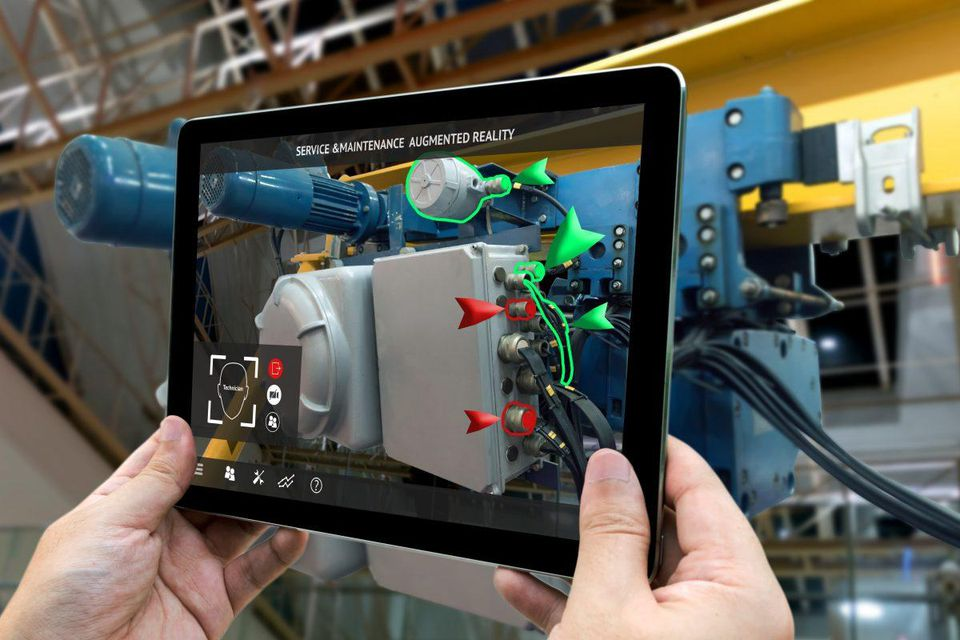
\includegraphics[width=0.6\linewidth]{imagenRAMantenimiento}
    \caption{Ejemplo de uso de la RA en servicios de mantenimiento.}
    \label{fig:googleglass}
\end{figure}

A continuación, se explicará en detalle:
\begin{itemize}
\item ¿Cómo funciona esta tecnología?.
\item Tipos de Realidad Aumentada.
\item Diferencias entre Realidad Aumentada y Realidad Virtual.
\item Realidad Mixta.
\item Futuro y usos de la Realidad Aumentada.
\item Integración de Realidad Aumentada en Android Studio.
\end{itemize}  

\subsubsection{¿Cómo funciona esta tecnología?}
La RA necesita de un dispositivo de visualización en el que mostrar esta unión del entorno real junto con la información digital. Esta unión puede ser visualizado en múltiples dispositivos: pantallas, gafas, dispositivos portátiles, dispositivos móviles, etc.
 
Además de estos sistemas de visualización, se necesita de un sistema de computación que realice los cálculos y reciba los datos provenientes de múltiples sensores, es decir: una CPU, una GPU, RAM, GPS, WIFI, bluetooth, acelerómetro, giroscopio, cámara, etc. Gracias a estos elementos el sistema puede reconocer el entorno real.

Todo esto necesita una parte software. El software en una primera parte deberá de reconocer el terreno, ubicaciones, objetos e imágenes, mediante los datos de los sensores y la cámara. Este proceso de transformación de diferentes conjuntos de datos a un sistema de coordenadas se llama registro de la imagen \cite{URL::ImageRegister}. 

Posteriormente el software deberá reestructurar el mundo real en función del registro de imágenes, añadiendo y combinando la información correspondiente al entorno para generar la imagen de RA. Existen múltiples maneras en las que se puede reestructurar este mundo. 

\begin{figure}[h]
    \centering
    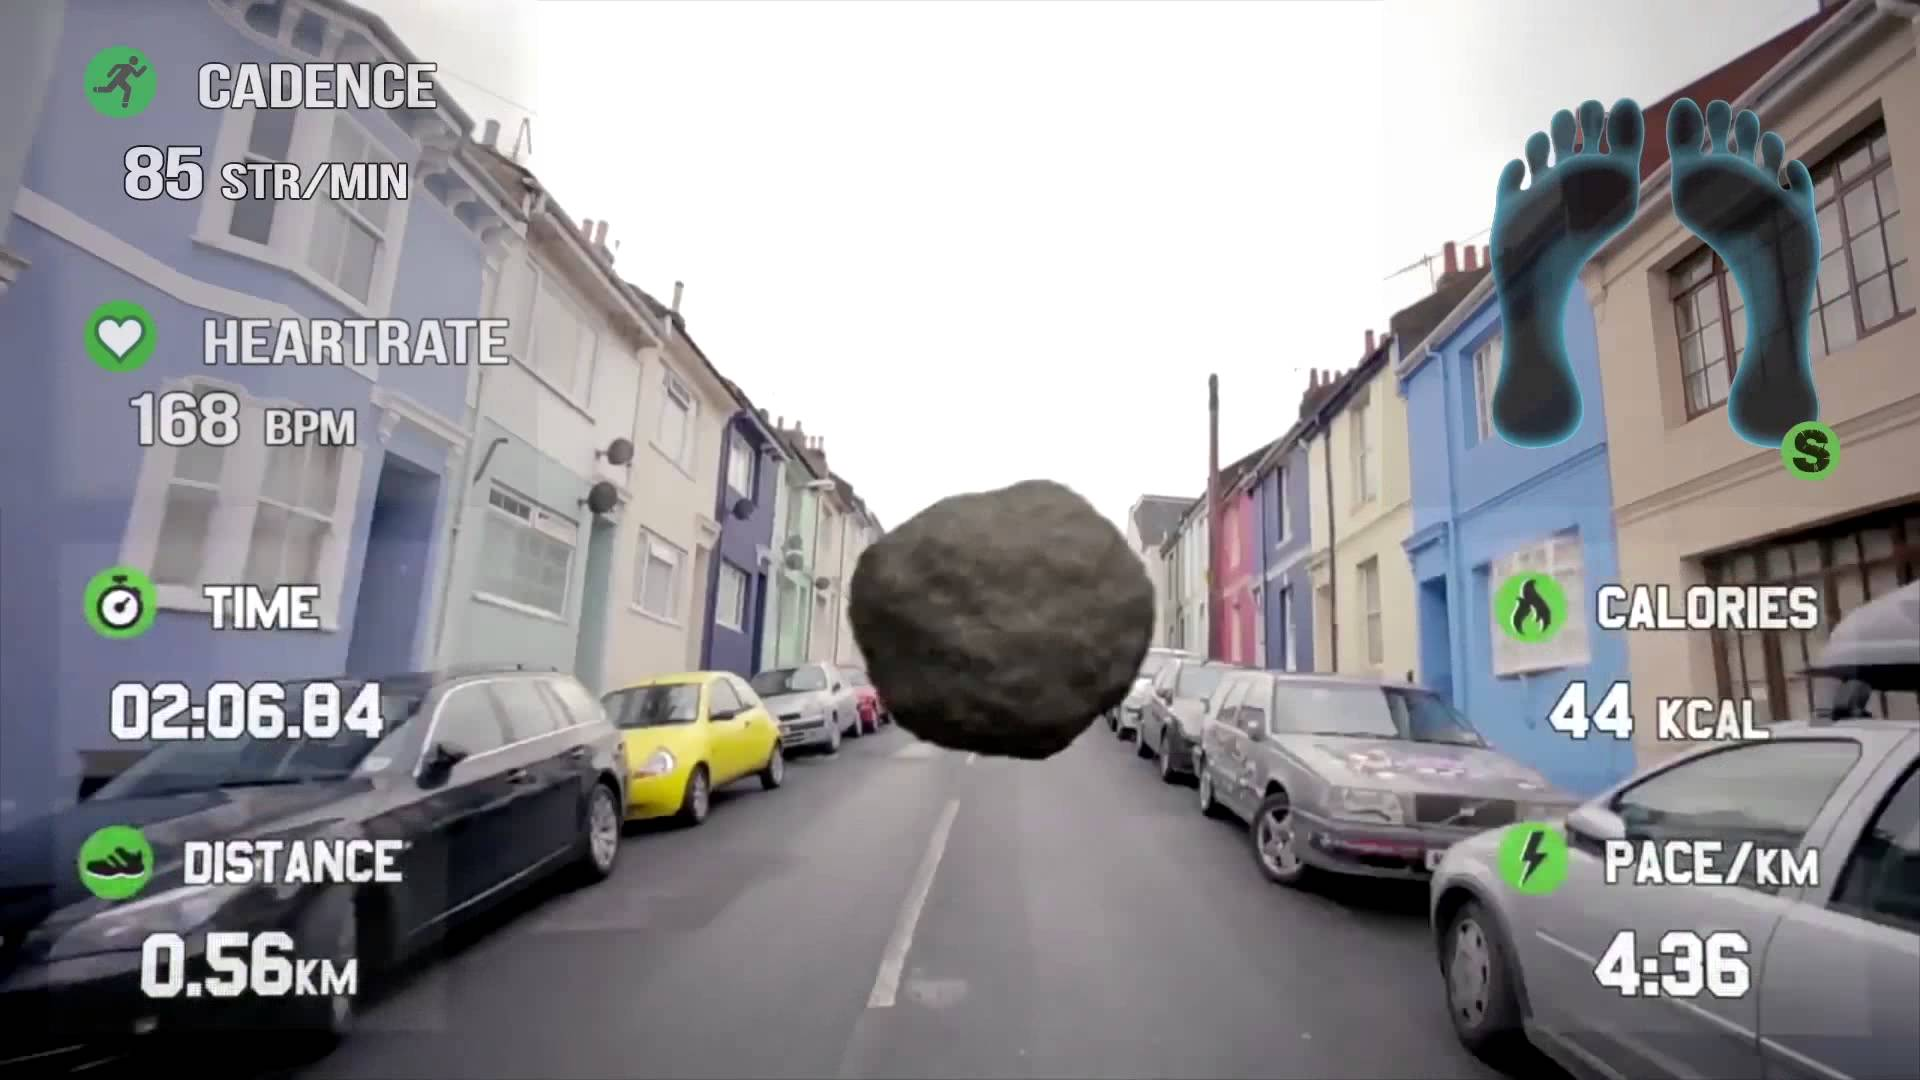
\includegraphics[width=0.6\linewidth]{googleglass}
    \caption{Google Glass. Desmostración del uso de RA en deportes.}
    \label{fig:googleglass}
\end{figure}

\subsubsection{Tipos de Realidad Aumentada}

Existen hoy en día cuatro tipos de RA:

\begin{itemize}
    \item 
    Marker-based AR. Se basa en el reconocimiento de imágenes conocidas como \textit{marker} o marcadores. 
		Los marcadores son imágenes distintivas que son reconocidas fácilmente por un dispositivo, debido a que contienen puntos visuales únicos. Un buen ejemplo de este tipo de imágenes son los conocidos códigos QR \cite{URL::CodigoQR}. Una vez se ha reconocido un marcador, se puede agregar información virtual. Esta información puede ser la incorporación de animaciones o vídeos en una página de un libro de texto, simulaciones de objetos 3D o arquitecturas sin llegar a construirlas de forma física (véase Figura \ref{fig:markerAR}).
    \begin{figure}[h]
        \centering
        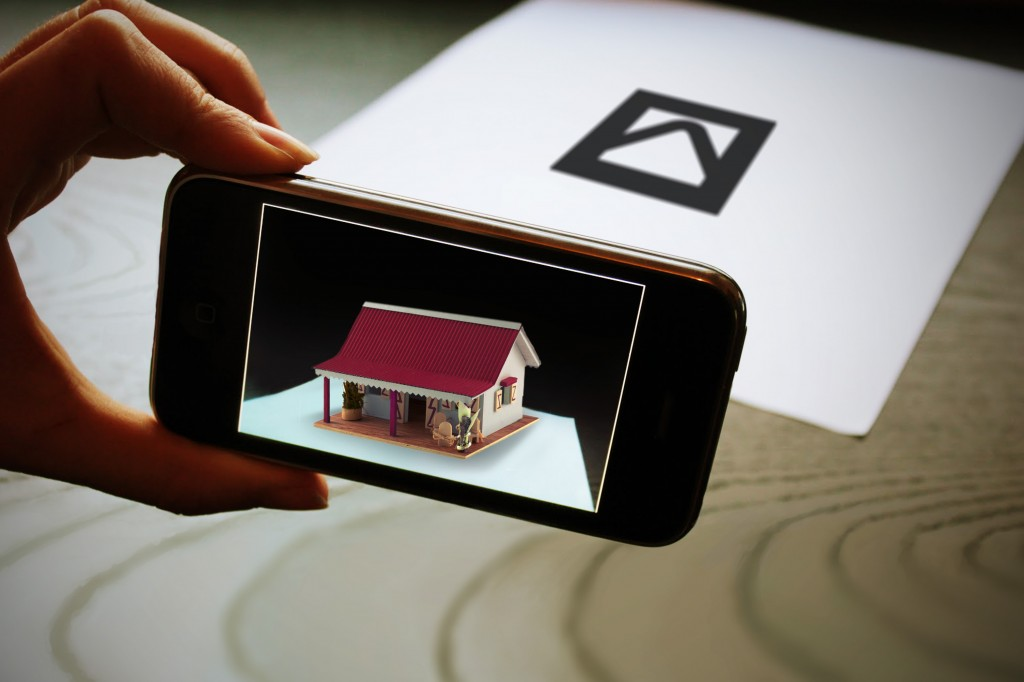
\includegraphics[width=0.6\linewidth]{marker-ar}
        \caption{Marker-bases AR. Demostración de su funcionamiento.}
        \label{fig:markerAR}
    \end{figure}

   

    \item Markerless AR. Corresponde a la RA que recoge los datos de su posición y orientación para mostrar la información correspondiente a esa área. Estos sistemas utilizan los datos obtenidos de la cámara, GPS, brújula, giroscopio y acelerómetro para establecer la ubicación del usuario en el entorno. Utiliza técnicas para reconocer terreno o ambientes para calcular la posición y orientación de la cámara. Con este tipo de tecnología se puede probar un mueble en el salón antes de llegar a comprarlo.

 
    \item Pojection-based AR. Este modo de RA consiste en la proyección de luz en superficies y objetos en el mundo real. Existen muchos usos interesantes de esta tecnología, como aplicaciones para el uso de teclados virtuales proyectados que reconozcan cuando una ``tecla" es pulsada. Esta proyección también se puede hacer en medio del aire con ayuda de la tecnología de láseres de plasma.

    \item Superimposition-based AR. Esta tecnología reemplaza la imagen original por una de RA, de forma completa o parcial. El reconocimiento de objetos juega un papel fundamental en este tipo de tecnología. Tiene gran utilidad el campo de la medicina, por ejemplo, un doctor podría examinar a un paciente mientras ve la imagen de RA que se creado a partir de una visión de rayos X y la imagen real de paciente, así puede ver y entender mejor el daño en un hueso.
\end{itemize} 

Aparte de los cuatro tipos de RA, existen subtipos dentro de cada uno de ellos.

``Location-based AR" es un tipo de ``Markerless AR"  que se centra más en los cálculos de la orientación y geolocalización del dispositivo. Esta técnica RA puede proveer de ayuda viajeros que necesiten una mano para moverse por la ciudad, ya que mediante el reconocimiento de su ubicación y la orientación pueden mostrarles la ruta para llegar a su destino o mostrarle información de los puntos de interés que les rodean. Esta será la técnica de RA implementada en la aplicación a desarrollar en este TFG. 


\subsubsection{Diferencias entre Realidad Aumentada y Realidad Virtual}
En los últimos años la realidad virtual (RV) \cite{URL::VR} o virtual reality (VR) en inglés y la realidad aumentada han empezado a recibir mucha más atención. Llevando a desarrolladores realizar integraciones de ambas tecnologías en numerosas industrias.

De acuerdo con un análisis de expertos, la RV iba tener el liderazgo en 2018 como tecnología pionera, sin embargo, la RA va a tener mucha más importancia y a largo plazo, llegará a formar parte del día a día.

La realidad virtual es un entorno de escenas u objetos de apariencia real. Aleja al usuario del entorno real y le brinda la sensación de estar inmerso en él. Dicho entorno es contemplado por el usuario a través de un dispositivo conocido como gafas o casco de realidad virtual. Este puede ir acompañado de otros dispositivos, como guantes o trajes especiales, que permiten una mayor interacción con el entorno, así como la percepción de diferentes estímulos que intensifican la sensación de realidad.

La realidad aumentada no aísla al usuario de mundo exterior, sino que traslada al mundo real objetos virtuales mediante la superposición de imágenes en tiempo real. 

\subsubsection{Realidad Mixta}

Existe otro tipo de tecnología que nace de la unión de realidad aumentada y la realidad virtual, la realidad mixta (RM) \cite{URL::RM}. Es un tipo de realidad similar a la realidad aumentada, pero con una idea más ambiciosa de mezclar lo real con lo virtual.

\begin{figure}[h]
    \centering
    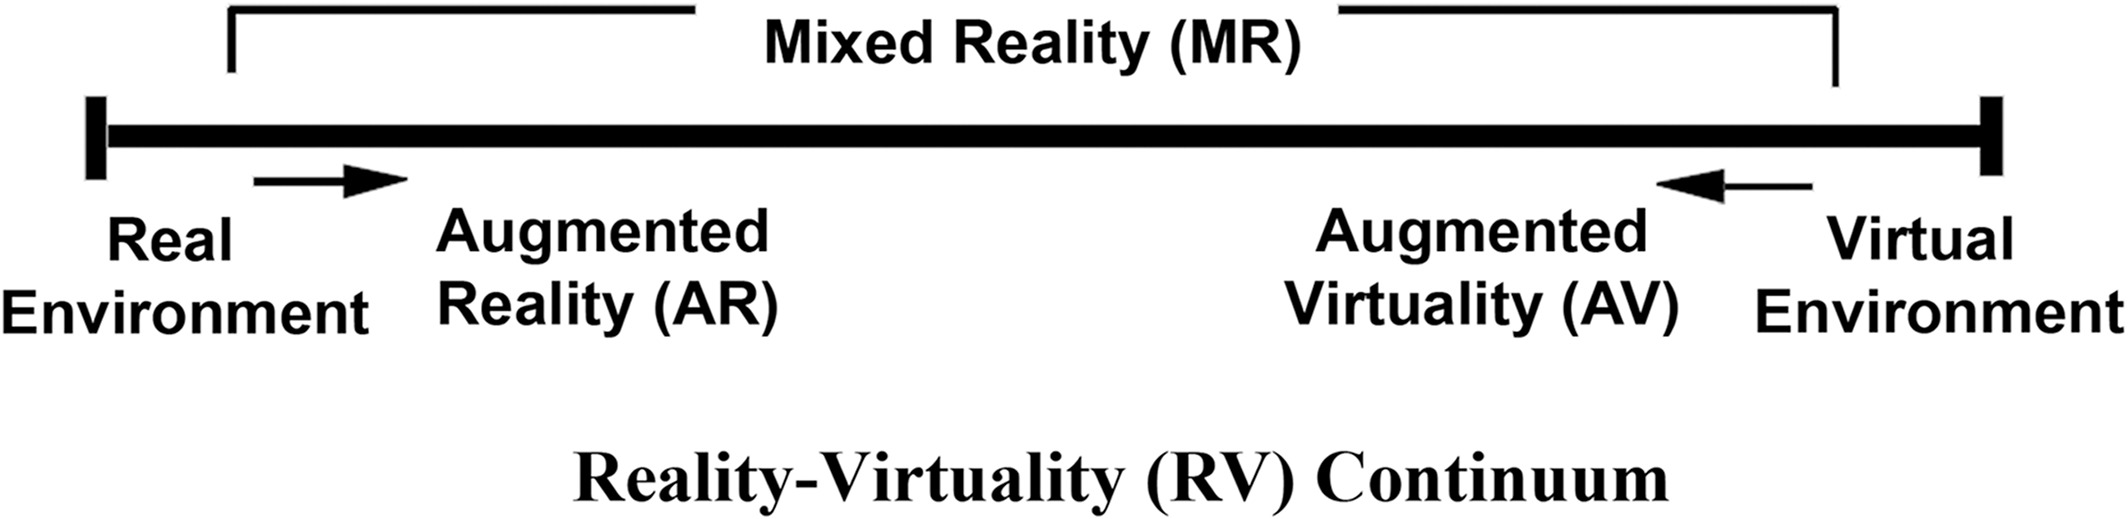
\includegraphics[width=0.6\linewidth]{realidamixta}
    \caption{ Espacio de la Realidad Mixta. }
    \label{fig:realidadMixta}
\end{figure}

En la RM se trata de llevar el mundo real al mundo virtual (véase Figura \ref{fig:realidadMixta}). La idea es generar un modelo 3D de la realidad y sobre él superponer información virtual. De esta forma, se podrán combinar ambas realidades para agregar contenido adicional de valor para el usuario de RM. La RM es mucho más inmersiva que la realidad aumentada y requiere de mucha más capacidad de procesamiento. 

\subsubsection{Futuro y usos de la Realidad Aumentada}
Actualmente la RA se encuentra más disponible a cualquier usuario, que en años anteriores. 
Dispositivos como los teléfonos móviles ya incorporan las primeras muestras de esta tecnología, la cual está aún en una fase inicial de desarrollo, pero ya se puede ver el potencial y la enorme importancia 
que va a cobrar en un futuro.

Los usos actuales de esta tecnología se acercan a todos los sectores conocidos:

\begin{itemize}
    \item Realidad Aumentada en educación. La llegada de la RA afectará a los procesos convencionales de aprendizaje. La RA tiene la capacidad de cambiar el horario y el lugar en el que se estudia y la posibilidad de introducir nuevos métodos de enseñanza. 
    
Actualmente gran parte de la población joven tiene un dispositivos móvil el cual es un medio idoneo para la RA. 
Por lo tanto, se dan unas condiciones adecuadas para que la RA profundice en el campo de la educación y se hagan más descubrimientos ya que cada estudiante va a tener un dispositivo a mano capaz de reproducir la RA, 
lo cual puede ayudar al alumnado a tener contenidos más accesibles sobre cualquier asignatura o conseguir que información compleja sea más fácil de entender. Un ejemplo claro sería la creación de libros interactivos que al ser apuntados con la cámara del móvil muestren el funcionamiento en 3D de un volcán (véase Figura \ref{fig:education-example}) o del latido de un corazón.

    \begin{figure}[h]
        \centering
        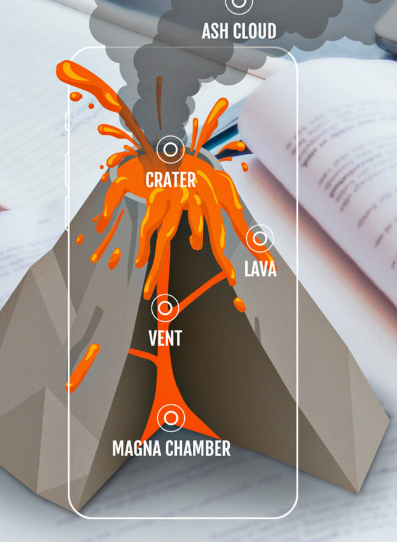
\includegraphics[width=0.35\linewidth]{education-example}
        \caption{RA Volcán. Ejemplo de uso de RA en Educación. }
        \label{fig:education-example}
    \end{figure}
    
    \item Realidad Aumentada en los videojuegos. Sin duda uno de los sectores en lo que más interés se tiene para desarrollar esta tecnología y quizás donde más se haya avanzado en realidad aumentada. Todas las grandes empresas de este sector tienen ya potentes desarrollos y lanzamientos de videojuegos que combinan la realidad física con la virtual, con múltiples posibilidades de personalización dentro de cada juego. En un futuro esta tecnología revolucionará todo el sector de los videojuegos y cambiará la manera en la que se interactúa con ellos.   
    
    Un claro ejemplo del potencial de la RA en este sector, está en el éxito de Pokemón Go! \cite{URL::Pokemon-Go}. Una aplicación para dispositivos móviles que utiliza técnicas de RA basadas en la localización, la cual a través de la cámara del dispositivo y modelos 3D para representar a los personajes de la saga Pokemón \cite{URL::Pokemon}, los cuales se encuentran escondidos en ubicaciones del mundo real.  
    
    
    
    \item Realidad Aumentada en la industria. El desarrollo de aplicaciones de RA en el ámbito industrial también está creciendo, ya que ayuda a mejorar la productividad de los ciclos de trabajo. Por ejemplo, algunas empresas están desarrollando aplicaciones que ayuden a los trabajadores de una cadena de montaje. De este modo, los empleados pueden obtener información adicional sobre las acciones que llevan a cabo. Este mismo sistema también se puede implementar en las reparaciones de vehículos o maquinaria industrial, ya que la aplicación puede mostrar toda clase de avisos sobre las piezas deterioradas. Incluso puede llegar a mostrar contenido visual en 3D sobre cómo llevar a cabo la reparación o sustitución de esos elementos. 
    

    \item Realidad Aumentada en turismo. El negocio turístico siempre ha intentado estar al día con la nueva tecnología para poder ofrecer nuevos servicios, formas de publicitarse, transporte y actividades de ocio. Por eso no es raro que la RA se haya hecho un hueco en este sector debido al potencial que tiene para mejorar la experiencia de los turistas. 
    
    La RA tiene la capacidad de generar aplicaciones que permitan a los turistas realizar una visita guiada por las ciudadades que visiten, permitiéndoles moverse sin problemas por la ciudad, señalando puntos de interés, datos históricos, restaurantes, hoteles, etc. El mismo concepto podría aplicarse en museos y zoos. Otro uso interesante sería el de romper la barrera del lenguaje gracias a la traducción inmediata de señales, textos y anuncios, al idioma del turista. Para los Juegos Olímpicos de Tokio 2020 se espera tener esta tecnología preparada para poder traducir a los visitantes en tiempo real todos los textos, señales y anuncios, a través de sus dispositivos móviles.   

    

    \item Realidad Aumentada en medicina. En cuanto a la medicina, es interesante ver cómo avanza la tecnología en este campo que sin duda apunta prometedor para mejorar la calidad de vida y salud de la población.
    
    Los principales usos que se plantean se encuentran enfocados principalmente en los quirófanos, en los que el especialista o cirujano monte una especie gafas-pantalla que le permitan realizar la operación sin la necesidad de apartar la vista del paciente para consultar información o ir monitorizando la operación. Esto se traduce en operaciones más rápidas y seguras sin que el cirujano se despiste. A su vez, esto podría mostrar información anatómica sobre el paciente en tiempo real, es decir, gracias a algoritmos de inteligencia artificial, permitir identificar nervios, venas mayores y huesos, y que estos sean marcados con un distinto color, facilitando mucho las labores de los médicos.

\end{itemize}

\subsubsection{Android Studio y la RA}


Para la integracion de realidad aumentada en Android, se han probado y estudiado los kits de desarrollo de software (SDK \cite{URL::SDK}) de realidad aumentada disponibles para Android Studio. Los SDK que han sido evaluados son:



\begin{itemize}
    
    \item  \textbf{Vuforia} \cite{URL::vuforia} es un SDK de realidad aumentada que permite a los desarrolladores de aplicaciones crear rápidamente experiencias de RA inmersivas, de alta fidelidad y centradas en el móvil. El SDK de Vuforia aprovecha la tecnología de visión por computadora para identificar y rastrear imagenes y objetos 3D en tiempo real. Esta funcionalidad permite orientar y colocar objetos virtuales, incluidos modelos 3D y otros contenidos, en relación con el entorno del mundo real. Los modelos 3D y la información digital se pueden superponer sobre la escena del mundo real y verlos en relación con el entorno a través de un dispositivo móvil.
    
Este SDK es uno de los mejores del mercado con buen soporte para aplicaciones multiplataforma. 
Un inconveniente de Vuforia es que está diseñado para desarrollar aplicaciones y juegos principalmente en plataformas como Unity \cite{URL::Unity}. 
En cuanto al SDK para Android Studio, la falta de soporte, de documentación y los númerosos problemas hallados a la hora de instalarlo, lo convierten en un SDK con el que nos ha sido muy difícil trabajar. 
Es por ello que se ha decidido descartar Vuforia para su integración en \ULLAR{}.

    \item \textbf{Kudan AR SDK} \cite{URL::kudan} es una plataforma diseñada para desarrolladores de RA como una plataforma preprada para admitir tanto en el reconocimiento basado en marcadores como sin marcadores y el seguimiento de de los mismos. 
El motor Kudan SDK principal, se desarrolla completamente en C++ y posee optimizaciones específicas de la arquitectura desarrolladas para proporcionar un rendimiento más rápido y sólido sin afectar negativamente el espacio de memoria. 
    
La instalación de Kudan AR fue rápida y sencilla, debido a que Kudan dispone de la documentación necesaria para instalarlo en Android Studio. 
Además, dispone de una guía bien explicada para comenzar la implementación de sus funcionalidades. 
Se ha optado por la integración de este SDK debido a su sencillez y a que ofrece los requisitos mínimos para el objetivo de RA de \ULLAR{}.

\item  \textbf{MaxST SDK} \cite{URL::maxst} de realidad aumentada proporciona un motor RA integral multiplataforma equipado con todas las características requeridas por los desarrolladores para crear experiencias y aplicaciones de RA. 
MaxST AR proporciona las siguientes funcionalidades: seguimiento instantáneo, SLAM \cite{URL::SLAM} (utiliza la cámara del teléfono inteligente para crear un ``mapa virtual'' del área circundante), rastreo de objetos y reconocimiento de imágenes y de marcadores.
    
MaxST AR ofrece unos de los mejores soportes para la integración de un SDK de RA en Android Studio. 
Dispone de  tutoriales en su página web para la instalación del SDK, explicando el funcionamiento e implementación de cada una de las funcionalidades que ofrece. 
No se le ha encontrado ningún inconveniente para integrarlo en la aplicación, pero se ha preferido integrar Kudan AR SDK por su simplicidad.
\end{itemize}

% Se ha optado por utilizar ``Kudan AR SDK" para el desarrollo de la aplicación de este TFG debido a problemas de compilación y flexibilidad en las opciones gratuitas de los otros dos SDK en Android Studio.  


\subsection{Node.js}

Node.js \cite{URL::Nodejs} es una librería y entorno de ejecución de E/S dirigida por eventos y por lo tanto asíncrona que se ejecuta sobre el intérprete de JavaScript creado por Google llamado Chrome V8 \cite{URL::ChromeV8}. Node.js es un entorno de JavaScript del lado del servidor \cite{URL::serverside}, basado en eventos. Utilizar el motor de Chrome V8 permite a Node.js un entorno de ejecución que compila y ejecuta JavaScript a velocidades increíbles.

Node.js fue desarrollado con el objetivo que fuera un sistema escalable y que tuviera la consistencia de generar un elevado número de conexiones de forma simultánea con el servidor. La mayoría de las tecnologías que de los servidores tradicionales tienden a accionar las peticiones de forma aislada y mediante hilos independientes. Esto se traduce en que a mayor número de solicitudes mayor es la cantidad de recursos necesarios para responderlas. Node.js se ha desarrollado para optimizar la gestión de estas solicitudes.

La solución que propone Node.js se basa en el tratamiento de las solicitudes de forma unificada en un único hilo complementado con un bucle de eventos de tipo asíncrono. De este modo cada petición que se recibe se trata como un evento y pertenecen a este único bucle (véase Figura \ref{fig:nodejsEx}). Este nuevo replanteamiento proporciona un lenguaje con una capacidad para gestionar una gran cantidad de solicitudes y conexiones con la máxima eficiencia.

Node.js utiliza un E/S de tipo asíncrono. En los modelos de tipo asíncronos, las tareas que efectúa el servidor se realizan de manera simultánea y repartidas entre los hilos del procesador. Este procedimiento evita que se produzcan bloqueos y proporciona una mayor potencia y velocidad de procesamiento.

     
\begin{figure}[h]
    \centering
    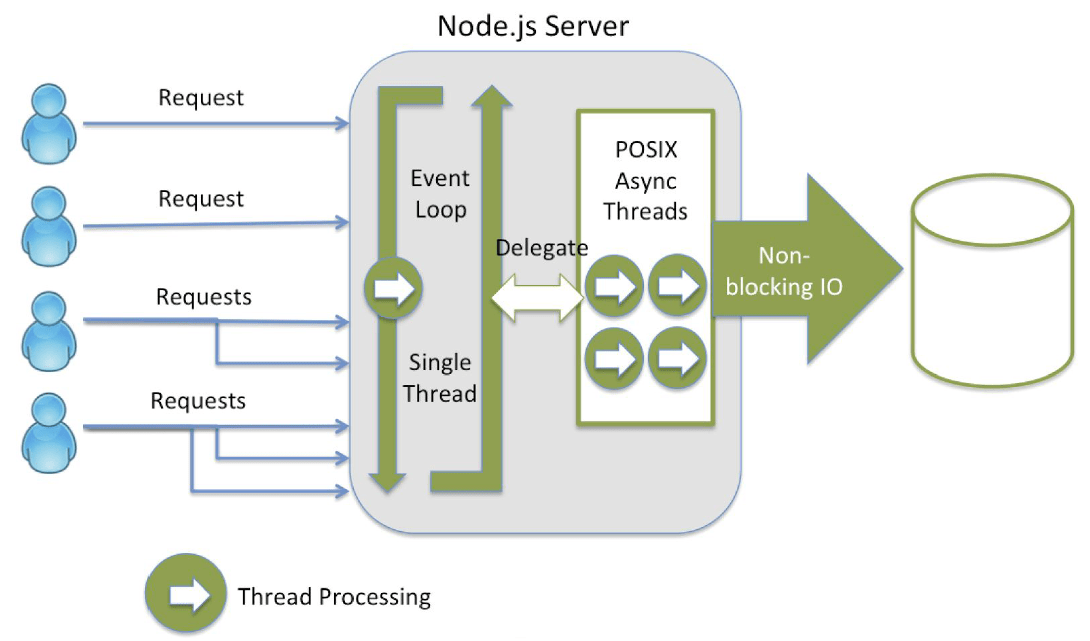
\includegraphics[width=100mm,scale=1]{nodejsEx}
    \caption{Funcionamiento de Node.js.}
    \label{fig:nodejsEx}
\end{figure}


% Para poder comunicarse con diferentes clientes el servidor se encarga de unas tareas denominadas E/S, las cuales hacen referencia a aquellas que están destinadas una entrada y salida de información. Un E/S de tipo sincrónica lo cuales se ejecutan las instrucciones de forma lineal, es decir una instrucción no se ejecuta hasta que la anterior no ha terminado de ejecutarse. Esto llevaba a el alargamiento innecesarios de algunos procesos de trabajo y a la tendencia de que se produzcan bloqueos. 

% JavaScript es un lenguaje cuyo principal uso se centra en el lado del cliente. Sin embargo Node.js está diseñado para ejecutar JavaScript desde lado del servidor. JavaScript es un lenguaje muy extendido entre los desarrolladores lo cual hace que Node.js sea una alternativa más sencilla. Pero esta no es la única razón por la que se eligió este lenguaje. Sus rasgos de lenguaje asíncrono y orientado al diseño de eventos ofrecían mejores condiciones para trabajar con él en esta arquitectura.   

Otro de sus puntos fuertes es su gestor de paquetes Node Package Manager  (NPM). Gracias a este gestor se pueden instalar paquetes, módulos y agregar dependencias de manera simple.

Se ha optado por el uso de un servidor que implemente la tecnología Node.js como servidor de \ULLAR{} por la facilidad  para ejecutar este servidor en cualquier tipo de sistema operativo y para su futura integración en la nube, 
gracias a la plataforma Heroku de la que se hablará más adelante. 
Otra de las razones por las que se ha elegido Node.js es porque el proceso de desarrollo y programación es rápido y sencillo y además se tenían conocimientos previos sobre esta tecnología, lo que ha facilitado su uso.


\begin{figure}[h]
\centering
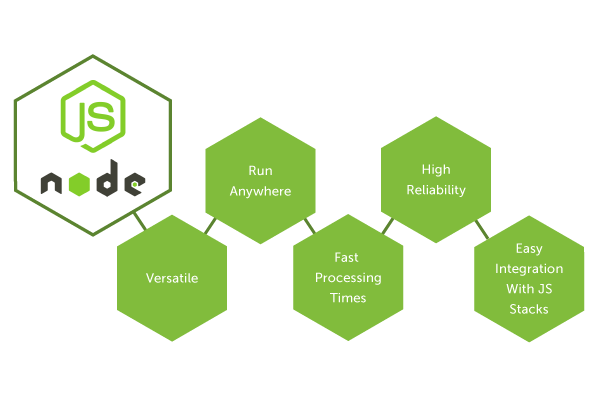
\includegraphics[width=115mm,scale=1]{nodejsfunc}
\caption{Ventajas de Node.js.}
\label{fig:nodejsVentajas}
\end{figure}

% \subsubsection{¿Porqué Node.js?}
% \begin{itemize}
%     \item Fácil de integrar e instalar en cualquier servidor, sin importar el sistema operativo.
%     \item JavaScript como base. Un lenguaje conocido por cualquier programador.
%     \item Gran rendimiento, permite generar a su vez arquitecturas potentes y sólidas.
%     \item Su alta capacidad de escalabilidad. La creación de aplicaciones web con la capacidad de atender muchos miles de solicitudes en un único servidor de forma simultánea, sin la necesidad de tener que incrementar las infraestructuras de servidores.
%     \item Un proceso de desarrollo y programación de aplicaciones rápido y liviano.
% \end{itemize}


Para instalar Node.js en una máquina con Linux se deben ejecutar estos comandos:
\begin{lstlisting}
    $ curl -sL https://deb.nodesource.com/setup_11.x | sudo -E bash -
    $ sudo apt install -y nodejs
\end{lstlisting}


% \subsubsection{ Desventajas }

% \begin{itemize}
%   \item Se desconoce el funcionamiento e implementación de Node.js en empresas de hosting.
%   \item La API es inestable en lo que respecta al cambio entre versiones.
%   \item Falta de Librerías en General. Dado que JavaScript no ha sido muy popular en el lado del servidor existe algunas librerías de las que carece en la actualidad.
%   \item Es bastante flexible en cuanto las formas en la que se puede programar. Pero esto genera bastantes problemas debido a la falta de organización en el código. 
% \end{itemize}

\subsection{MongoDB}

\subsubsection{ Descripción }

MongoDB  \cite{URL::MongoDB} es un sistema de base de datos multiplataforma NoSQL   \cite{URL::NoSQL} orientado a documentos. Esta base de datos es de esquema libre, es decir, al contrario que las bases de datos relacionales no utilizan una tabla fija para guardar la información.

Un registro en MongoDB es un documento, cuya estructura de datos se compone por el par campo y valor. Utilizan un formato para guardar estas estructuras que se llama BSON  \cite{URL::BSON} también llamada JSON \cite{URL::json} Binario. Este formato tiene una ventaja pese a que puede ocupar más espacio de lo que lo haría el formato JSON. BSON guarda de forma explícita las longitudes de los campos, los índices de los arrays, y demás información útil para el escaneo de datos y así agilizar las búsquedas en estos documentos.

Estos documentos, que a su vez incorporan una clave primaria como identificador, son la unidad básica de datos en MongoDB. Las colecciones en MongoDB contienen un conjunto de documentos y funciones equivalentes a las de las bases de datos relacionales.

Debido a los requisitos de la aplicación, el uso de una base de datos de MongoDB
permitía la creación de una base de datos de esquema libre, es decir, sin la preocupación de crear tablas de datos para almacenar la información, que permitía guardar de forma simple toda la información necesaria para 
el funcionamiento de la aplicación. 
Además, las consultas a esta base de datos se facilitan con el uso de un servidor Node.js, que ofrece un conjunto de librerias y paquetes preparados para realizar la comunicación con una base de datos de MongoDB.

% La consola de mongo es una interfaz interactiva de JavaScript la cual permite a los usuarios de MongoDB consultar, actualizar y administrar estas bases de datos. Esta consola es un componente estándar de las distribuciones de Open Source.

\begin{figure}[h]
    \centering
    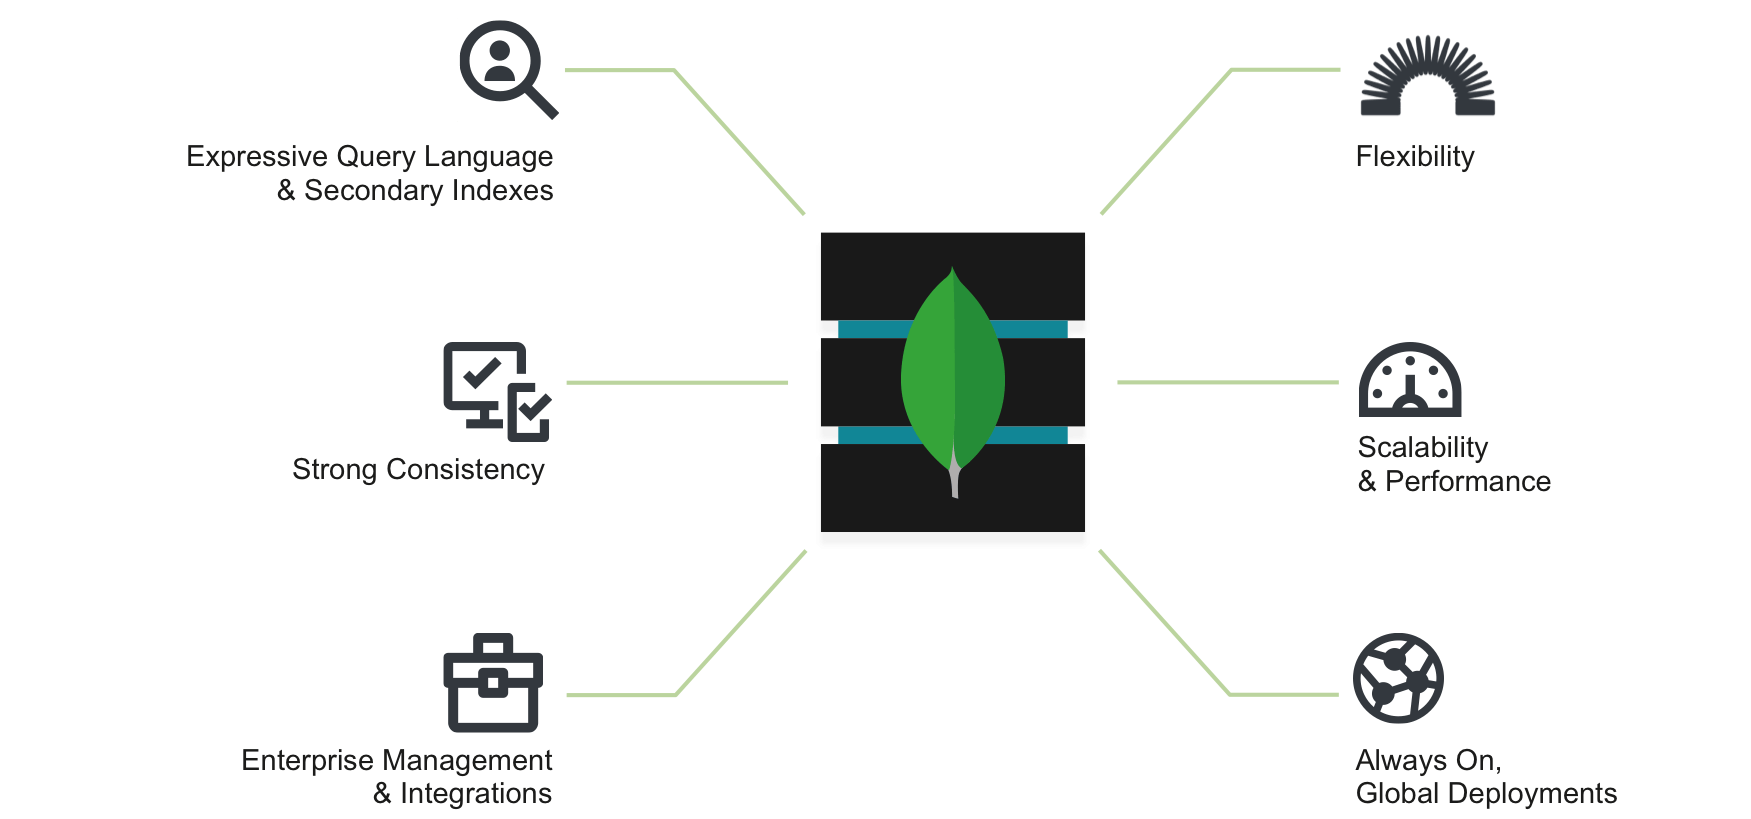
\includegraphics[width=150mm,scale=2]{mongodb-architecture}
    \caption{ Ventajas de MongodDB. }
    \label{fig:mongoDBarquitectura}
\end{figure}


% \subsubsection{ Ventajas de MongoDB }


% \begin{itemize}
    
%     \item El hecho de que sea una base de datos NoSQL, significa que no necesita esquemas predefinidos y puede guardar cualquier tipo de datos. Esto otorga una gran flexibilidad para crear cualquier tipo de campos que se necesiten en un documento, permitiendo mayor escalabilidad en MongoDB comparado a las bases de datos tradicionales.

%     \item A su vez, el uso de documentos para guardar la información hace que sea mucho más fácil de mapear estos datos en los lenguajes nativos de programación.

%     \item Es fácil  acceder a los documentos si se indexan. En MongoDB este indexado provee de rápidos tiempos de respuesta a las peticiones, esto le permite ser hasta 100 veces más rápido que los modelos de bases de datos relacionales.

%     \item MongoDB es una base de datos distribuida, por lo que es fácil de usar y proporciona una elevada disponibilidad, escalabilidad horizontal y distribución geográfica.
    
 
% \end{itemize}

% Por otro lado existen una serie de inconvenientes y limitaciones:

% \begin{itemize}
%   \item No soporta las consultas SQL ya existentes. Un ejemplo de esta es la consulta Join \cite{URL::JoinSQL}, la cual supone una desventaja en cuanto a rendimiento si se tienen que añadir manualmente los datos en el caso de querer realizar una consulta de este tipo.

%   \item No es una solución adecuada para aplicaciones con transacciones complejas.
%   \item Falta de estandarización entre las diferentes bases de datos NoSQL.
% \end{itemize}

\subsection{ Heroku }

Heroku es una plataforma como servicio de computación (PaaS \cite{URL::PaaS}) en la nube que soporta distintos lenguajes de programación. Heroku permite a desarrolladores y compañías construir, proporcionar, monitorizar y escalar aplicaciones. Es una forma sencilla de montar una infraestructura en la nube.

Heroku es conocida por ejecutar las aplicaciones en ``dynos". Un dyno es simplemente un ordenador virtual que pueden ser encendido y/o apagado en función del tamaño y requisitos de la aplicación.

A cada uno de estos dynos se le puede configurar más espacio o capacidad de procesamiento, o se pueden añadir más dynos si la aplicación lo necesita. Heroku a cada mes realiza un cobro en función de los dynos que el usuario tenga contratados. 

Se ha optado por utilizar el dyno gratis que ofrece Heroku a cada repositorio. El cual tienen un límite de 1000 horas activas al mes y se pone en suspensión a los 30 minutos sin recibir tráfico. Una vez que vuelve a recibir tráfico se activa de nuevo.   

Se ha utilizado Heroku para albergar el servidor de \ULLAR{}, ya que ofrece un servicio gratuito idóneo para el diseño de pequeñas aplicaciones web en la nube, sin la complejidad de estar implementando un servidor físico. 

Para instalar Heroku basta seguir las indicaciones que se hallan en \cite{URL::HerokuCLI}.


\subsection{ mLab }
mLab es un servicio de base de datos en la nube totalmente gestionado que ofrece aprovisionamiento y escalados automáticos de las bases de datos MongoDB, copia de seguridad y recuperación, monitoreo, herramientas de administración basadas en web y soporte experto. La plataforma de base de datos como servicio de mLab corre sus máquinas en proveedores de servicios en la nube como AWS \cite{URL::aws}, Azure \cite{URL::Azure} y Google Cloud \cite{URL::GoogleCloud}.

En esta plataforma se ubicará la base de datos de \ULLAR{}. 
Dadas las facilidades de acceso a ella e integración con el servidor de la aplicación en Node.js, es una opción simple, fácil de manejar y con posibilidad de escalar.

\subsection{ Google Maps }

La API de Google Maps \cite{URL::GoogleMapsApi} fue publicada para Android en 2008 y en 2012 para IOS. Esta API permite utilizar mapas basados en datos de Google Maps en una aplicación Android, y además ofrece métodos para personalizar el mapa:
\begin{itemize}
    \item Creación de marcadores, polígonos y superposiciones sobre el mapa para resaltar puntos o zonas. 
    \item Permite cambiar la vista del usuario de modo que se muestre un área del mapa en particular. 
    \item Ofrece la posibilidad de elegir el tipo de mapa: de carreteras, satélite, híbrido (fusión de carretera y satélite) y de terreno.
\end{itemize}

Esta API fácil de integrar y con soporte de Google, es la mejor opción para tener un mapa funcional y que permita ubicar al usuario de la aplicación.
